\section{Environmental security}

When considering building a launch pad facility for spaceflights, there is a lot
of work to do before starting the actual building. The launch pad is something
that would be strongly subjected to environmental conditions and they would have a
great impact in the final performance of the launch pad and the risk factor of
that the rockets would suffer.

For that, the first important thing to take into account when building a
spaceport is the election of the more suitable place to build it. In this way,
other factors are also involved:

\begin{itemize}
	\item The proximity to equator to minimize cost of orbital insertion for equatorial orbits.
	\item The existence of inhabited areas around the launch pad, ideally sea.
	\item Low risk of earthquakes and tsunamis.
	\item Good communications by airports or seaports.
	\item Good atmospheric conditions; natural protection against winds, tornadoes...
\end{itemize}

Let's assume that we have some places that equally good in terms of position respect
to the equator, they all have inhabited areas around it, low earthquake risk and
good communications. In this case we just have to decide the better place according
to the last point: the atmospheric environment.

The atmospheric conditions that a spaceport may withstand could be very variable
and they could affect a lot the launch of the rocket, which would impact on the
cost of the launches, if, for example, delays are needed, or even worst, there
is a launch failure during or before the launch.

\subsection{Atmospheric security}

In this section, what we are considering is the prevention against atmospheric
phenomena around launchpads. Atmospheric conditions involves a large number of
phenomena: winds, rains, snow, storms and lightnings, temperature changes, humidity, air pressure.

The first point to decide whether a place is appropriate for a launch pad is what
we are going to call the \textbf{passive atmospheric security}. That is, the
ways that the place is naturally protected against atmospheric phenomena. This is
something that could not be changed. Because of that, the former election of the
place is very important, because after you decide a place, this conditions
are not expected to change anymore.

On the other side, we would refer to \textbf{active atmospheric securty} to
all the security measures that we would intentionally design in order to improve
the passive ones.

In our study we will focus on the active protection systems, more particularly
in lightening protection system. Let's assume that we have good enough passive
protection against winds, rains and so on. But, as we'll see later, even having
selected the best place in terms of atmospheric conditions, is mandatory to
install this lightning security systems because every single place is subjected
to possible storms and/or lightenings.

Moreover, as said previously, the election of the launch pad use to prefer places
near a large body of water, like the sea. It’s known that the coastline use to be
a zone with higher lightening impact rate. And furthermore, a launch pad, having
in their surrounding water and other flat terrains, use to be, always, the highest
point in a large area, having heights of about 60-100 m., making them more prone
to a cloud-to-ground lightning strike.

The prevention against lightenings is very important because it’s proven that
they could damage both the rocket and the launch pad facilities, or at least,
they can power on some systems on the rocket or in the launch facilities that
may cause unexpected delays or damages. Given that, it’s clear that a good
protection system is required in every launch pad.

As explained before, its mandatory to provide some lightning protection system to
launch pads. This system shall be able to \cite{RONGIER201327}:

\begin{itemize}
	\item Intercept or divert all dangerous downward flashes away from the launch pad.
	\item Control the electric potential voltage of the environment around the
	rocket and also the soil around the launch pad to be within safe limits.
	\item Limit the electromagnetic field in the volume of the launchpad.
\end{itemize}

Given that the height of the launch pads use to be not high enough to have significant upward lightning activity, the main protection is focused only for downward strikes.

\subsection{Present Lightning Protection Schemes}

Nowadays there are some different approaches on the design of that lightning
protection systems for launch pads. The next figure \ref{fig:towers}\cite{RONGIER201327}, shows some
of them.

\begin{figure}[h!]
	\centering
	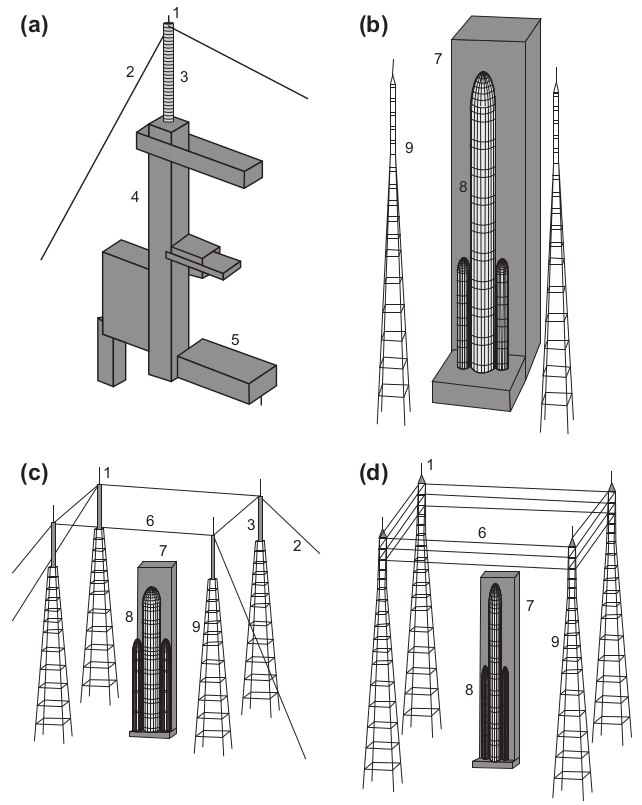
\includegraphics[width=\textwidth]{img/launchpad_towers.png}
	\caption[Launch pad lightning protection system schemes]
	{1 Lightning rod, 2 Catenary/Ground wire, 3 Insulating mast, 4 Fixed Service Structure, 5 Launch pedestal , 6 Shield wires, 7 Umbilical Tower, 8 Launch Vehicle, 9 Towers.}
	\label{fig:towers}
\end{figure}

The scheme shown in figure (a) is relatively simple, as it just uses the fixed
service structure as a tower to put the lightning rod on top of it, using an
insulating mast between it and the the tower structure. Then, to derive the
electric current of the strike, one or two stainless steal cables run from the
lightning rod to remote earthing points. This is the scheme used in some launch
pads currently in use like John F. Kennedy Space Center 39A, in figure \ref{fig:39a}.

\begin{figure}[h!]
	\centering
	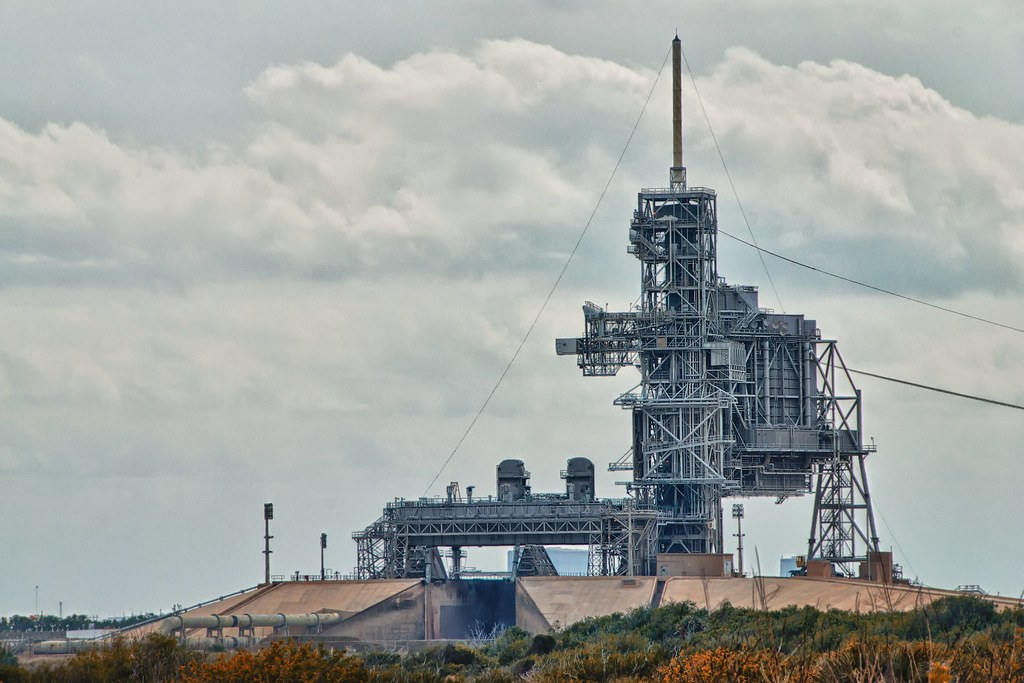
\includegraphics[width=0.7\textwidth]{img/39a.jpg}
	\caption{Launch pad 39A lightning protection system}
	\label{fig:39a}
\end{figure}

Other structures (c and d) include cables between the towers to create a box,
that acts like a Faraday cage helping reducing the electromagnetic fields that
could exists within the atmosphere. That is for example, the scheme used in
Kourou (French Guyana) launch pad for ESA, depicted in image \ref{fig:ariane5_towers},
during a launch of Ariane 5.

\begin{figure}[h!]
	\centering
	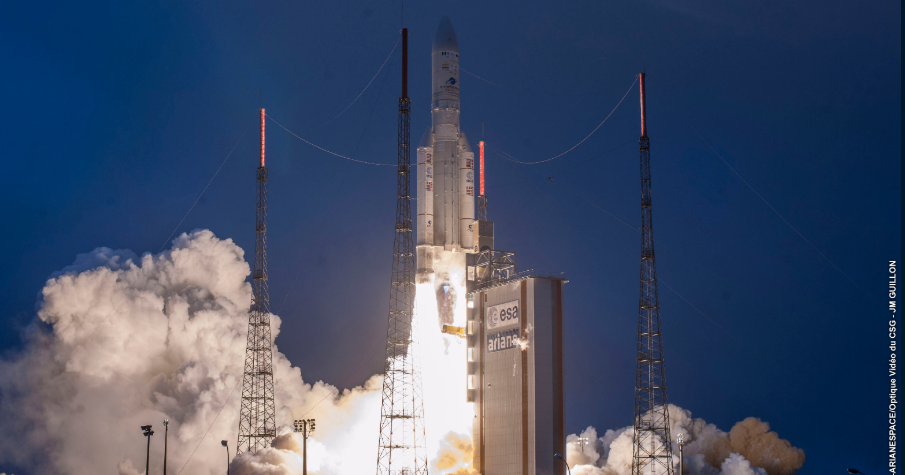
\includegraphics[width=0.7\textwidth]{img/ariane5_towers.png}
	\caption{Kourou Space Center launch pad towers during a launch of an Ariane 5}
	\label{fig:ariane5_towers}
\end{figure}

\subsection{Designing methods of lightning protection systems}
\subsubsection{Rolling sphere method}

For the correct design of the towers and the position of the lightning rods, the
usual way to do it is by the rolling sphere method. In that method, a virtual
sphere of a radius defined by the level of protection desired, is made roll around
the whole structure always with one or more points in contact with the
structure we want to protect. All the point that the sphere is touching during the
roll, are the points that are directly exposed to be hit by a strike. The ones that
aren't touched are protected from them. Next picture \ref{fig:rsm} shows how this
method works \cite{2012Issac}.

\begin{figure}[h!]
	\centering
	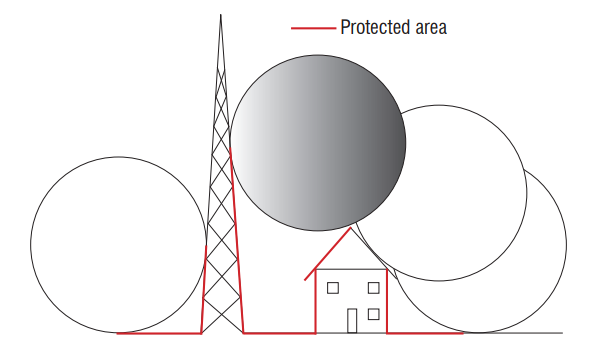
\includegraphics[width=0.7\textwidth]{img/Rolling_sphere_method.png}
	\caption{Rolling sphere method. The red parts of the drawing are protected from lightnings}
	\label{fig:rsm}
\end{figure}

But this method is not accurate enough always, and it should be used just as a
initial approach in the design of the protective system. After that, more accurate
and precise calculations should be taken into account.

But, even that, the physics of the ray propagation through the atmosphere is still
quite difficult and is very difficult to predict where would be the attachment
points on any structure. Some recent experiments have shown that, for example,
very sharp structures are less effective than more rounded shapes;
this could be due to the sharpness of the object ensures a large intensification of the
field, but it also creates a charge that shields the lightning rod itself, making it
ineffective \cite{2004RISON}.

\subsubsection{Experimental models}

Other way to study the design of this protection system is by experimentally testing
in a laboratory with a scaled model of the rocket and the launch pad towers and
rods, and generating electric discharges. This was used for the design of the ZL3
launching pad at the Guyana Space Center (CSG) using a 1/20 scale model structure
of the launching pad (figure \ref{fig:model_ariane}).

\begin{figure}[h!]
	\centering
	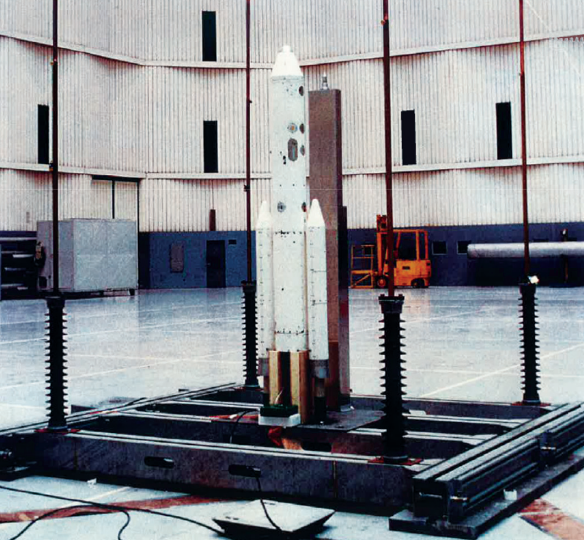
\includegraphics[width=0.7\textwidth]{img/model_ariane.png}
	\caption{Scale model of Ariane 5 launch pad}
	\label{fig:model_ariane}
\end{figure}

But, even that, this way of measuring the effectivity of the protection system
design, could be not completely adequate because the conditions inside the laboratory
could be faked or not equal to the actual, natural environmental conditions. The
real simulation of that conditions inside a laboratory could be quite difficult.

This is why the design of the lightning for spaceports is done almost exclusively
using the electro-geometric model, as defined in the international standard procedures
for typical buildings. However, these approaches cannot guarantee a total reliability of the
launching pad lightning protection system

With respect to the CEI 62305 standard \cite{ligthning_standard}, the most constraining
protection level is "LPL I" 3 kA, which gives a radius of 20 m for the rolling sphere,
and that's the one typically used in spaceports design.

In other cases, it can be used a bigger protection level, for example that was used
for Soyuz launch pad, showed in the figure \ref{fig:soyuz_sphere}. In this case
for a current of 5 kA and a 30 m rolling sphere, the standard gives
a Type II protection level, but this solution was found as the best
compromise between a direct lightning strike of 5 kA on the rocket
and a high level lightning strike of 200 kA on the LPS.

\begin{figure}[h!]
	\centering
	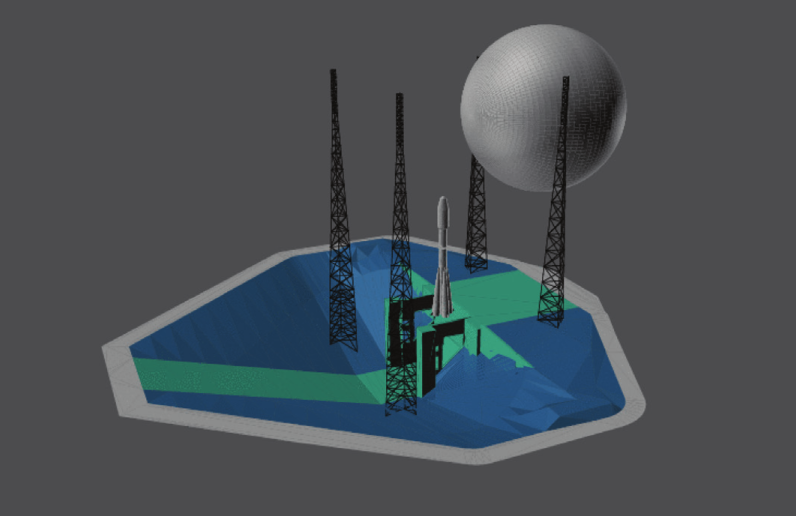
\includegraphics[width=0.7\textwidth]{img/soyuz_sphere.png}
	\caption{Rolling sphere method applied to Soyuz launch pad in French Guyana}
	\label{fig:soyuz_sphere}
\end{figure}
